% Created 2022-10-12 mié 19:16
% Intended LaTeX compiler: pdflatex
\documentclass[12pt]{article}
\usepackage[utf8]{inputenc}
\usepackage[T1]{fontenc}
\usepackage{graphicx}
\usepackage{grffile}
\usepackage{longtable}
\usepackage{wrapfig}
\usepackage{rotating}
\usepackage[normalem]{ulem}
\usepackage{amsmath}
\usepackage{textcomp}
\usepackage{amssymb}
\usepackage{capt-of}
\usepackage{hyperref}
\usepackage[spanish]{babel}
\usepackage{graphicx,geometry}
\geometry{ a4paper, left=1in, right=1in, top=1in, bottom=1in }
\renewcommand\familydefault{\sfdefault}
\usepackage{sectsty}
\sectionfont{\normalfont\Large }
\subsectionfont{\normalfont}
\usepackage{tabularx}
\usepackage{listings}
\lstdefinestyle{mystyle}{
numbers=left,
showspaces=false,
frame=leftline,
showspaces=false,
showstringspaces=false,
showtabs=false,
numberstyle=\tiny,
}
\lstset{
style=mystyle,
literate={á}{{\'a}}1
{é}{{\'e}}1
{í}{{\'{\i}}}1
{ó}{{\'o}}1
{ú}{{\'u}}1
{Á}{{\'A}}1
{É}{{\'E}}1
{Í}{{\'I}}1
{Ó}{{\'O}}1
{Ú}{{\'U}}1
{ü}{{\"u}}1
{Ü}{{\"U}}1
{ñ}{{\~n}}1
{Ñ}{{\~N}}1
{¿}{{?``}}1
{¡}{{!``}}1
}
\makeatletter
\usepackage{fancyhdr}
\pagestyle{fancy}
\usepackage{mdframed}
\BeforeBeginEnvironment{minted}{\begin{mdframed}}
\AfterEndEnvironment{minted}{\end{mdframed}}
\author{Luis Eduardo Galindo Amaya (1274895)}
\date{07-10-2022}
\title{Instrucciones de transferencia y aritmeticas.}
\hypersetup{
 pdfauthor={Luis Eduardo Galindo Amaya (1274895)},
 pdftitle={Instrucciones de transferencia y aritmeticas.},
 pdfkeywords={},
 pdfsubject={},
 pdfcreator={Emacs 26.3 (Org mode 9.1.9)}, 
 pdflang={Spanish}}
\begin{document}



\newcommand{\docente}{Arturo Arreola Alvarez}
\newcommand{\asignatura}{Organización de Computadoras (331)}
\newcommand{\semestre}{2022-2}

\newcommand{\miportada}[1]{
	\begin{titlepage}
		\vspace*{0.75in}
		\begin{flushleft}
			\sffamily
			\large #1       \\
			\Huge 
            \@title         \\
			\hrulefill
			\vspace{0.25in} \\
			\Large \@author \\
			\vspace*{\fill}
            
\includegraphics[width=\textwidth]{../includes/filler.png} \\
			\vspace*{\fill}
			\large
			\begin{tabular}{|l|l|}
              \hline
			  Asignatura & \asignatura \\
			  Docente    & \docente    \\
			  Fecha      & \@date      \\
              \hline
			\end{tabular}
		\end{flushleft}
	\end{titlepage}
}

\miportada{ Práctica 7 }

\fancyhf{}
\lhead{ \asignatura }
\rhead{ \semestre }
\rfoot{Página \thepage}

\setlength\parindent{0pt}   % eliminar el intentado
\setlength{\parskip}{1.2em}
\maketitle

\section*{Instrucciones}
\label{sec:org66e33e7}
\subsection*{Objetivo}
\label{sec:org566b8cd}
Seleccionar las instrucciones aritméticas y de transferencia de datos
adecuadas para desarrollar aplicaciones de sistemas basados en
microprocesador mediante la distinción de su funcionamiento, de forma
lógica y ordenada.

\subsection*{Desarollo}
\label{sec:org925951a}
\subsubsection*{Parte 1}
\label{sec:org303170a}
Descargue el archivo print\_hex.asm proporcionado en la plataforma. Abra Google Colab y ensamble el código con NASM por medio del comando:

\begin{verbatim}
nasm -f elf print_hex.asm
\end{verbatim}

Encadene el archivo con la librería utilizando el siguiente comando:

\begin{verbatim}
ld -m -elf_i386 print_hex.o <PATH_de_la_libreria> -o print_hex
\end{verbatim}

El cual generará el archivo ejecutable print\_hex. Ejecute el archivo por medio del comando:

\begin{verbatim}
./print_hex
\end{verbatim}

Pruebe el programa colocando diferentes valores en EAX para entender el funcionamiento del mismo.

\subsubsection*{Parte 2}
\label{sec:orgf6b4fb5}
Cree un programa llamado P7.asm que contenga la rutina print\_hex, la cual recibe en EAX un valor que se quiere imprimir en formato hexadecimal. Agregue a P7.asm las instrucciones necesarias para hacer lo que se indica a continuación:

\begin{itemize}
\item a. Coloque en EBX el valor 0x5C4B2A60. Sume su matrícula como valor hexadecimal. Si su matrícula es 12345678 expresarla como 0x12345678. Almacene el resultado en EBX.

\item b. Coloque los 16 bits menos significativos de EBX en la pila.

\item c. Defina una variable N de 2 bytes de longitud. En ella, guarde el resultado de la multiplicación de BL por 8, sin considerar los signos.

\item d. Incrementar en 1 el valor guardado en N.

\item e. Divida el valor almacenado en BX entre 0xFF. Imprima tanto el cociente como el residuo de la operación.

\item f. Realice la suma entre el valor almacenado en N y el residuo de la división anterior. Guarde el valor en N y decremente N. Realice las operaciones necesarias para imprimir el registro de banderas y explique que banderas están activas y porque.

\item g. Saque un dato de 16 bits de la pila.
\end{itemize}

\begin{verse}
NOTA: Por cada inciso, despliegue en pantalla el nuevo valor del registro modificado utilizando la subrutina print\_hex.\\
\end{verse}

\pagebreak


\section*{Desarollo de las actividades}
\label{sec:orgd7a9dc9}
\subsection*{parte 1}
\label{sec:org4bc7f1f}

\begin{center}
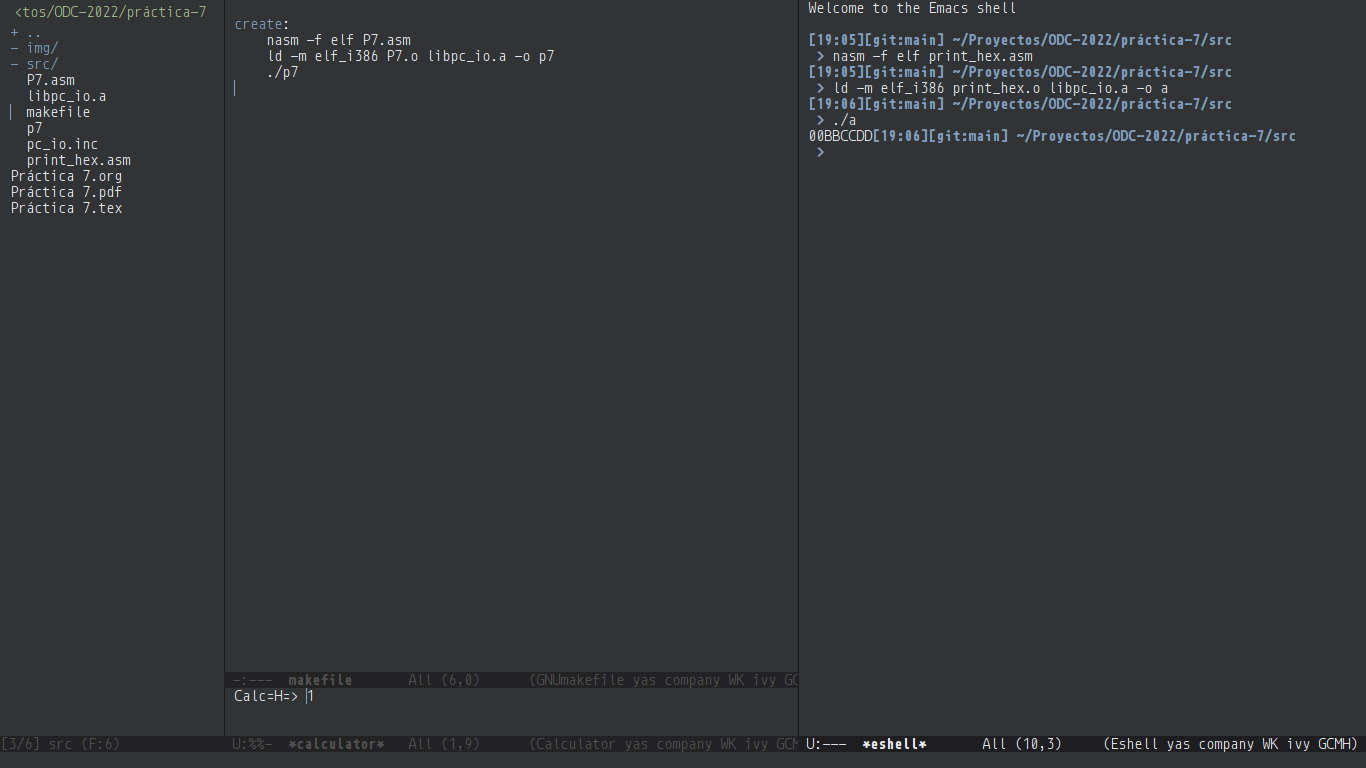
\includegraphics[width=7cm]{img/1.png}
\end{center}

El programa se pudo compilar con los siguiente comandos:
\begin{verbatim}
nasm -f elf print_hex.asm
ld -m elf_i386 print_hex.o libpc_io.a -o a
./a

00BBCCDD
\end{verbatim}

\subsection*{parte 2}
\label{sec:org8cc082a}
\subsubsection*{código}
\label{sec:org509b4b8}
\\ \lstinputlisting{./src/P7.asm}

\subsubsection*{Foto}
\label{sec:org92d4c64}
\begin{center}
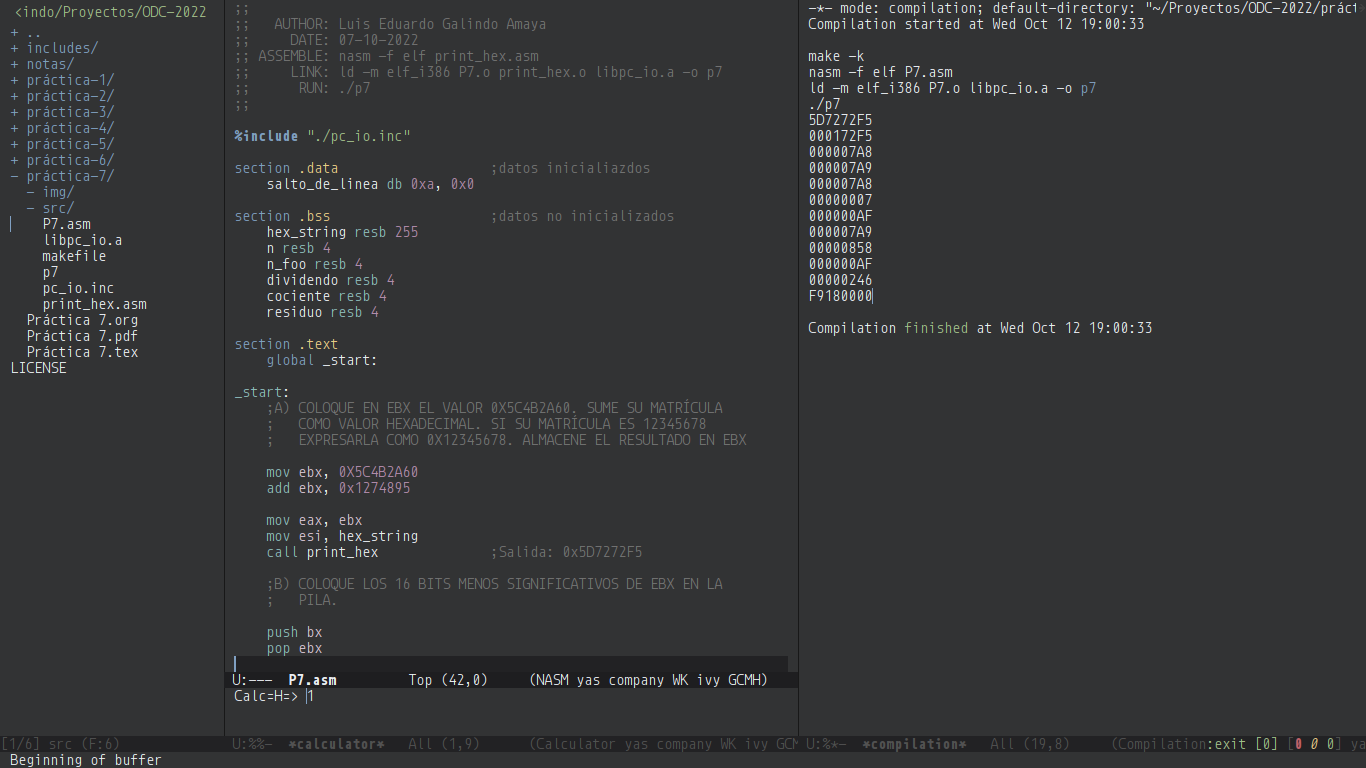
\includegraphics[width=7cm]{img/2.png}
\end{center}

\section*{Conclusiones y comentarios}
\label{sec:org3c344c5}
Fue muy interesante ver como hacer operaciones en ASM es bastante diferente de otros lenguajes, y entender por que la pila es tan útil para las operaciones matemáticas.

\section*{Dificultades en el desarrollo}
\label{sec:orgc7584d5}
Imprimir los valores del hex en la pantalla daba problemas, pude resolver parcialmente el error extendiendo el tamaño de string\_hex a 255 y haciendo que todas mis variables fueran de 4 bytes.
\end{document}
